\documentclass[doc, a4paper, apacite]{apa6}

\usepackage[american]{babel}

\usepackage{csquotes}
%\usepackage[style=apa,sortcites=true,sorting=nyt,backend=biber]{biblatex}
%\DeclareLanguageMapping{american}{american-apa}
\usepackage{threeparttable}
\usepackage{booktabs} % For nice tables
\usepackage{amsmath} % For \text{} function 
\usepackage{setspace}

\title{Decision-making and communication under uncertainty}
\shorttitle{DSTL07: Speaker to message}

\author{Charlotte E. R. Edmunds, Adam Harris, Magda Osman}
\affiliation{Queen Mary, UCL, University of London \\ 11 January 2021}

%\leftheader{Edmunds}

%\abstract{}
%
%\keywords{}

\begin{document}
	\doublespacing

\section{Method}

\subsection{Participants}
Participants will be recruited through Prolific academic.
Participants will be paid for their participation. 
Specifically, they will be given a flat fee for the training phase and a bonus depending on their score in the first test phase. 
% Power analysis

\subsection{Category structure}
The abstract category structure that participants will learn is shown in Table~\ref{table:abstractStructure}. 
The stimuli are constructed from five binary dimensions. 
In the experiment, Category X and Y will be randomly assigned to the labels `Friendly' and `Hostile.' 
In addition, the dimensions will be randomly assigned to the label (and therefore perceptual features) of Craft (airplane, submarine), Speed (fast, slow), Direction (left, right), Type (autonomous, decoy) and Status (fully operational, damaged). 
Participants will be told about these stimulus dimensions in advance. 

\begin{table}
	\centering
	\caption{}
	\label{table:abstractStructure}
	\begin{tabular}{lllllllllll}
		\toprule
		\multicolumn{5}{c}{Category X} &  & \multicolumn{5}{c}{Category Y} \\
		\cline{1-5} \cline{7-11} \\
		D1   & D2   & D3   & D4  & D5  &  & D1   & D2   & D3   & D4  & D5  \\
		\midrule
		1    & 1    & 1    & 1   & 1   &  & 0    & 0    & 0    & 0   & 0   \\
		1    & 1    & 1    & 1   & 0   &  & 0    & 0    & 0    & 0   & 1   \\
		1    & 1    & 1    & 0   & 1   &  & 0    & 0    & 0    & 1   & 0   \\
		1    & 1    & 1    & 0   & 0   &  & 0    & 0    & 0    & 1   & 1   \\
		1    & 1    & 0    & 1   & 1   &  & 0    & 0    & 1    & 0   & 0   \\
		1    & 1    & 0    & 1   & 0   &  & 0    & 0    & 1    & 0   & 1   \\
		1    & 1    & 0    & 0   & 1   &  & 0    & 0    & 1    & 1   & 0   \\
		1    & 0    & 1    & 1   & 0   &  & 0    & 1    & 0    & 0   & 1   \\
		1    & 0    & 1    & 0   & 1   &  & 0    & 1    & 0    & 1   & 0   \\
		0    & 1    & 1    & 1   & 0   &  & 1    & 0    & 0    & 0   & 1   \\
		\bottomrule
	\end{tabular}	
\end{table}

% TODO fix figure formatting
\begin{figure}
	\centering
	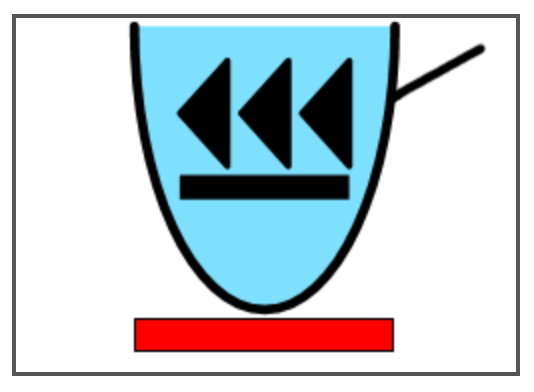
\includegraphics[width=0.33\textwidth]{images/integratedStimulusExample}
	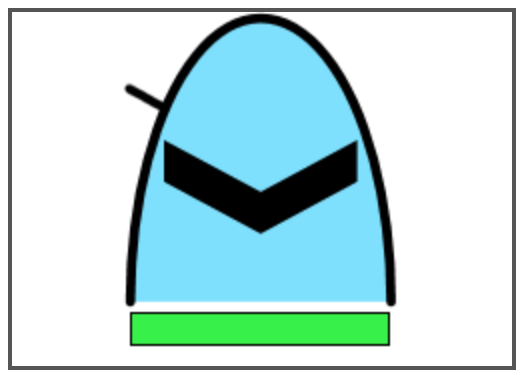
\includegraphics[width=0.33\textwidth]{images/integratedStimulusExample2}
	\caption{Example of stimulus dimensions as integrated stimuli.}
	\label{fig:integratedStimuli}
\end{figure}

\subsection{Design}
The experiment has a 2 (spatial presentation: separated, integrated) x 2 () between-subjects design. 

Participants will either see the stimuli as spatially integrated (as in Figure~\ref{fig:integratedStimuli}) or separated (as in Figure~\ref{fig:separatedStimulus}). 

\begin{figure}
	\centering	
	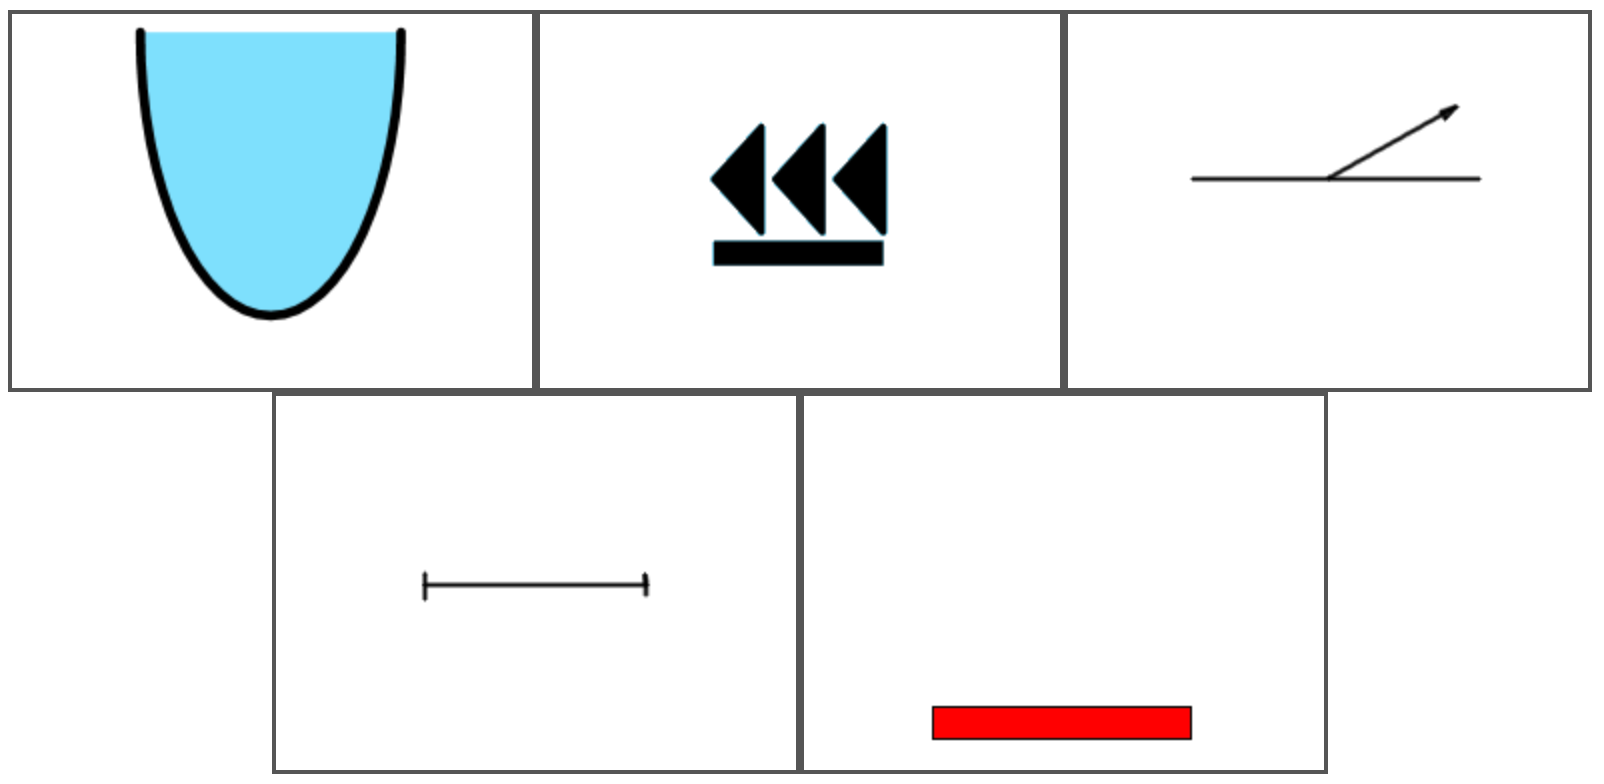
\includegraphics[width=0.5\textwidth]{images/separatedStimulusExample}
	\caption{An example stimulus presented as a separated set of symbols.}
	\label{fig:separatedStimulus}	
\end{figure}

This experiment has a two by two between-subjects experimental design. 
Participants will either see the stimulus dispersed or integrated. 
Additionally, they will be told that their confidence ratings are to be given to their commander or to one of their fellow operators. 

\subsection{Procedure}
At the beginning of the experiment, participants are welcomed and told where to write to if they have any queries or concerns. 
The experiment has three blocks of trials: a learning phase and two types of test phase. 

\subsubsection{1. Category learning} 
Participants are told the over all structure of the experiment, and then given specific instructions for the category learning phase. 
Additionally, they are told what each of the perceptual features of the glyph represent. 
On each trial, they are shown a radar screen with randomly placed diamond markers representing craft available on radar. 
One of those vessels is highlighted in red and enlarged. 
Then, depending on condition, participants either see an integrated glyph or a diagram where each of the elements are separated. 
They must decide whether the craft is friendly or hostile, and to respond they must press the `F' or `H' key respectively. 
Participants in this phase are trained to a learning criterion. 
This will likely be around 80\% but we need to check to see whether that is sensible. 





\clearpage
\newpage
\bibliographystyle{apacite}
\bibliography{references}

\end{document}
